\documentclass{jsarticle}
\usepackage[dvipdfmx]{graphicx}
\begin{document}
\thispagestyle{empty}
\begin{center}
{\huge 卒~~業~~論~~文のテンプレート}
\vspace*{3.5cm}

{\LARGE\bf cubing暗号の提案}
\vspace*{3cm}

{\large 20XX年X月提出日}
\vspace*{3cm}

{\large 立命館大学 情報理工学部}
\vspace*{5mm}

{\Large 石~川~~琉~聖}
\end{center}
\newpage 

\setcounter{page}{1}

\section*{概要}

研究論文の内容について、500 - 600 字程度でまとめる。
この概要を読めば、大体どういうことを研究したのかがわかるように書く。
具体的には、どういう問題について、どのような研究を行って、その結果どのような
結論が得られたか、というポイントについて簡潔にまとめる。

\newpage

\tableofcontents
\clearpage

\section{はじめに}
暗号がここらへんで使われててそこそこ大事って言う社会的背景を語る

\section{準備}
\subsection{記号の定義}
\subsection{暗号化とは}
ここは「1.はじめに」に含んでも良さそう
先に下を書き,この用語の説明が必要と言ったものがあれば書く

\section{本論}
\subsection{cubing暗号の概要}
cubing暗号の概要は以下の通りである.
\begin{itemize}
  \item 平文ブロック長:45byte
  \item 暗号文ブロック長:108byte
  \item 鍵長:可変
  \item 暗号化処理の並列化:可 (※但し,Shuffle処理がボトルネックとなる)
  \item 復号処理の並列化:可 (※但し,Sort処理がボトルネックとなる)
  \item Random Read:不可
\end{itemize}
なお,cubing暗号は暗号利用モード「cubingmode(CBGモード)」の利用を前提とし,以下cubing暗号に対しcubingmodeを利用した際の手順を説明する.
\subsection{cubing暗号の暗号化・復号手順}

以下の順序で暗号化・復号を行う.

\subsubsection{暗号化}
\noindent
1. 平文をブロックに分ける.\\
2. 必要があればパディングを用意する.\\
3. 全ての平文に対してマスク処理を行う.\\
4. 全てのブロックに対し,エンコードを行う.\\
5. 全てのブロックの平文以外の箇所に対してマスク処理を行う.\\
6. ブロックごとに暗号化を行う.\\
7. ブロックをシャッフルする.\\

\subsubsection{復号}
\noindent
1. 暗号文をブロックに分ける.\\
2. 全てのブロックに対して復号を行う.\\
3. 暗号化の(5)で使用したマスク処理を元に戻す.\\
4. (3)により現れるシーケンス番号を元に,ブロック間ソートを行う.\\
5. 暗号化の(3)で使用したマスク処理を元に戻す.\\
6. 全てのブロックに対し,デコードを行う.\\
7. 全てのブロックを結合させ,平文を生成する.\\

\subsubsection{パディング処理}
平文ブロックが45Byteに満たない場合,1Byte分null入れ,残りはランダムな英数列を入れる.これにより,平文を45Byteに固定することができる.

\subsubsection{コンピュータ上での表現方法}
ルービックキューブをコンピュータ上で表現する際には配列を用いる.具体的には以下のルービックキューブの展開図と配列の添字が対応する.\\

\begin{center}
  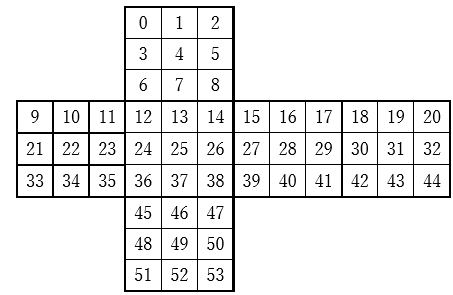
\includegraphics[width=7cm]{./tex_pic/seq.jpg}\\
\end{center}
    
\subsubsection{転置の仕様}
cubing暗号転置処理は方向・列・回数の三つより決定される.方向に関しては以下の図のように三種類定義される.縦方向はルービックキューブで処理する際,以下の図のように回転させる方向のことである.なお,図には各方向に対する列が記載されている.
\begin{center}
  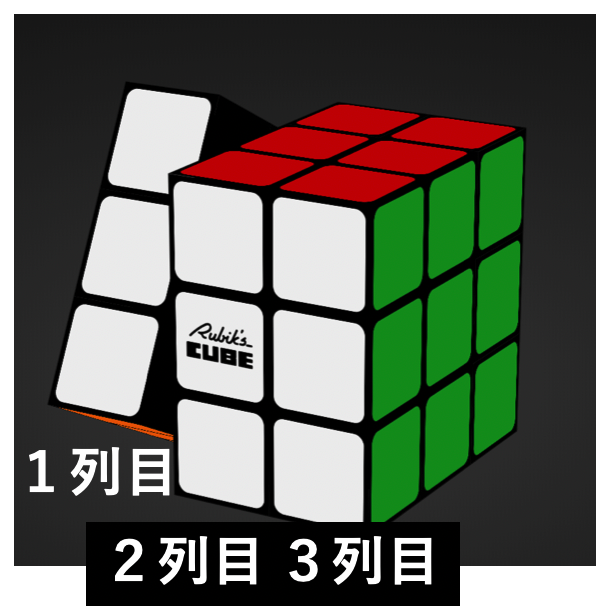
\includegraphics[width=7cm]{./tex_pic/tate.jpg}\\
(画像は http://iamthecu.be/ より引用)\\
\end{center}
横方向に関しては以下のように定義されている.
\begin{center}
  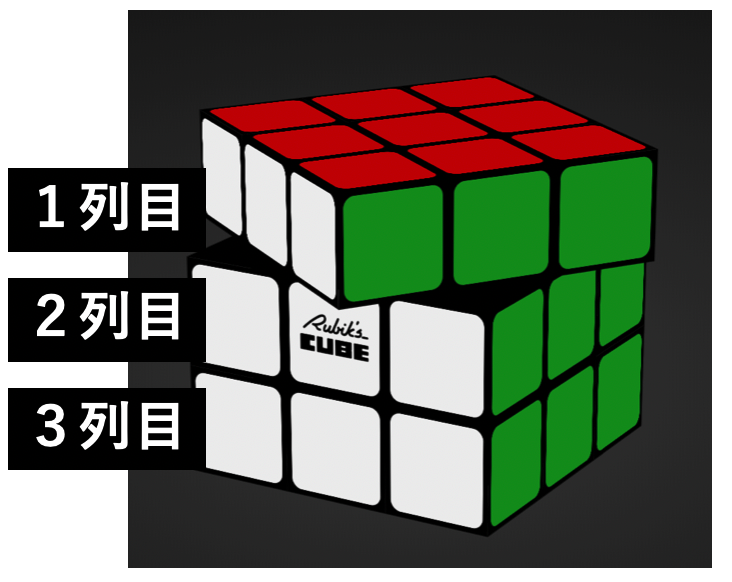
\includegraphics[width=7cm]{./tex_pic/yoko.jpg}\\
(画像は http://iamthecu.be/ より引用)\\
\end{center}
回転方向に関しては以下のように定義されている.
\begin{center}
  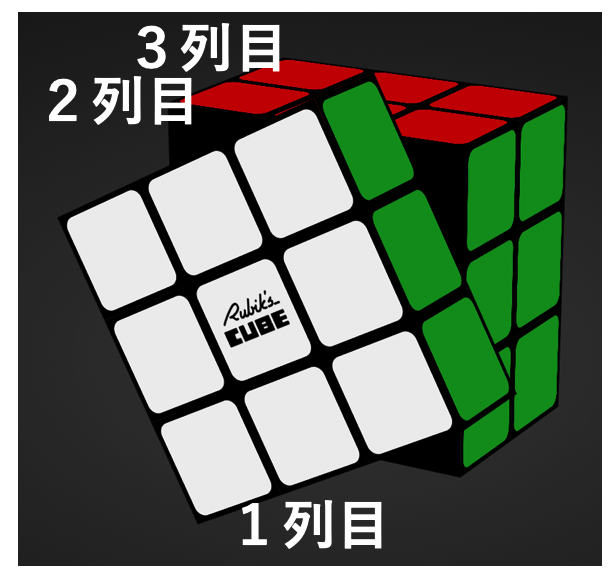
\includegraphics[width=7cm]{./tex_pic/kai.jpg}\\
(画像は http://iamthecu.be/ より引用)\\
\end{center}

なお,cubing暗号の転置はルービックキューブの転置とは一部違った箇所がある.それは,「ある方向のある列を転置させる際,他の列およびマスは一切転置させない」ということである.具体的には以下の図のような転置がなされる.\\
\\
//暇な自分へ\\
「1」「2」「3」\\
↓\\
「2」「3」「1」\\
みたいな図入れて\\

これにより,「ルービックキューブの角は常に同じ文字が隣り合っている」といった性質がなくなり,後述の頻度分析による解読の対策となる.


\subsubsection{暗号文の取得}
最後に,暗号文は以下の図の順で取り出す.
\begin{center}
  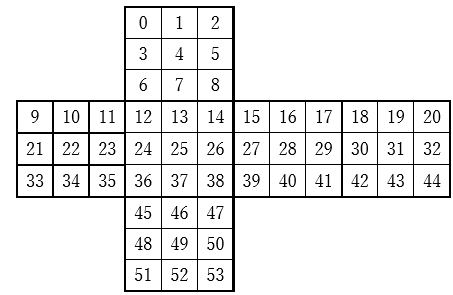
\includegraphics[width=7cm]{./tex_pic/seq.jpg}\\
\end{center}
\subsection{cubingmodeの利用手順}
\subsubsection{暗号化・復号の流れ}
\subsubsection{62進数の説明}
\subsubsection{エンコード処理}
\subsubsection{表示可能文字}
\subsubsection{mask(1)処理}
\subsubsection{mask(2)処理}
\subsubsection{encrypt処理}
\subsubsection{decrypt処理}
\subsubsection{shuffle処理}
\subsubsection{sort処理}
\subsubsection{送信内容}
\subsubsection{ブロック数が多い時の対策}

\section{評価実験}
ここでは主に長所を実験結果をもとに書く
\subsection{推奨する鍵の長さに関して}
鍵の長さを変えた時,転置されている割合を計算
\subsection{AES・RSAとの実行時間の比較}
具体的なやり方は考えておらず,おそらくOpenSSLなるものを活用することになる
\subsection{攻撃対策}
\subsubsection{ブルートフォース攻撃}
ここは計算量示すだけ
\subsubsection{頻度分析}
これより下はできないことを証明する
\subsubsection{選択平文攻撃}
\subsubsection{replay攻撃}
\section{関連研究}
\subsection{関連研究1(仮)}
\subsection{関連研究2(仮)}
\subsection{関連研究3(仮)}
\section{まとめ}
\subsection{まとめ1(仮)}
\subsection{まとめ2(仮)}
\subsection{まとめ3(仮)}
\section{謝辞}

\newpage 
%% 参考文献テンプレ

\begin{thebibliography}{}

\bibitem{長尾} 長尾真:知識と推論,岩波講座ソフトウェア科学14 (1988). 

\bibitem{実近} 実近憲昭: ゲームと AI,人工知能学会誌 vol.5, pp.527-537, 1990.

\end{thebibliography}

\end{document}
